\chapter{SDN Data Plane and OpenFlow}\label{ch:chapter5}
\section{SDN Data Plane}
Con il termine SDN Data Plane spesso ci si riferisce al livello infrastrutturale ovvero il livello dopo i dispositivi connessi alla rete performano il trasporto e il processo dei dati in accordo con le decisioni prese dall'SDN Control Plane. 
\newline
La caratteristica chiave dei dispositivi connessi alla rete nell'SDN � che questi ultimi performano una semplice funzione di inoltro dei dati senza bisogno di software che prendano decisioni al loro posto. 

\subsection{Funzioni del Data Plane}
Le principali funzioni dei dispostivi network sono le seguenti:
\newline
- \textbf{Control Support Function}: interagisce con il livello di controllo dell'SDN per supportare la porgrammabilit� attraverso l'interfaccia di risorse e controllo. Gli switch comunicano con il controller comunica con gli switch attraverso il protocollo OpenFlow degli switch. 
\newline
- \textbf{Data Forwarding Function}: accetta i flussi di dati provenienti da altri dispositivi network per inoltrarli sulle strade che sono state predefinite in accordo con il livello applicativo dell'SDN. 
\newline
Queste regole di instradamento utilizzate dai dispositivi network sono rappresentate dalle tabelle di instradamento che indicano per determinate categorie di pacchetti qual'� il loro prossimo passo da fare all'interno della rete.

\subsection{Protocollo del Data Plane}
Il protocollo � supportato da tutti i dispositivi network. Il flusso dei pacchetti dati consiste nel flusso di pacchetti IP; pu� quindi essere necessario per le tabelle di instradamento definire le entrate nei campi ad alto livello dei pacchetti, come avviene nel TCP o nell'UDP. La rete esamina l'IP header ed altri possibili header in ogni pacchetto per prendere le decisioni di instradamento. d

\section{OpenFlow}
Per tradurre il concetto di SDN nella implementazione pratica devono verificarsi due condizioni:
\newline
- deve essere presente una architettura logica comune fra gli switch, i router e gli altri elementi della rete; inoltre il tutto deve essere controllato da un controller SDN.
\newline
- un protocollo standard e sicuro � necessario tra il controller SDN ed i dispositivi network.
\newline
Questi requisiti sono indirizzati dall'OpenFlow, il quale � sia un protocollo tra l'SDN ed i dispositivi della rete che una specifica logica degli switch facenti parte della rete. Ogni switch � infatti in grado di connettersi agli \textbf{OpenFlow switches} e possibilmente il tutto si connette direttamente ai dispositivi finali che sono fonti o destinazione del flusso di pacchetti. Dalla parte degli switch l'interfaccia � nota come \textbf{OpenFlow Channel} e queste connessioni avvengono tramite le Open Flow ports che servono anche per connettere gli switch al controller SDN.
\newline
OpenFlow ridefinisce tre tipi di porte:
\newline
- \textbf{Pyhsical Port}: corrispondono all'interfaccia hardware degli switch
\newline
- \textbf{Logical Port}: queste porte non corrispondono direttamente a qualche componente hardware degli switch. Le porte logiche sono infatti delle astrazioni che possono essere definite negli switch utilizzando dei metodi non-OpenFlow (link, tunnel, loopback interface). Possono includere l'incapsulamento dei pacchetti e possono mappare varie porte fisiche. � necessario che interagiscano con il processo OpenFlow cos� come fanno le porte fisiche.
\newline
- \textbf{Reserved Port}: definite da specifiche OpenFlow. Specificano regole generiche di instradamento come l'invio e la ricezione dal controller o l'inoltro utilizzando metodi non-OpenFlow, come fanno gli switch normali.
\newline
\newline
Le specifiche OpenFlow definiscono tre tipi di tabelle bell'architettura logica degli switch:
\newline
- \textbf{flow table}: abbinano pacchetti in ricezione ad un particolare flusso e specificano quale tipo di funzione deve processare i pacchetti. Ci possono essere pi� tabelle di flusso che operano nella pipeline.
\newline
- \textbf{group table}: le flow table possono dirigere il flusso alle group table che possono intraprendere una variet� di azioni che va ad inficiare uno o pi� flussi di pacchetti.
\newline
- \textbf{meter table}: � in grado di innescare una moltitudine di azioni in un flusso di pacchetti. 
\newline
\subsection{Flow Table Structure}
Il blocco principale dell'architettura logica degli switch sono le flow table. Ogni pacchetto che entra in uno switch passa attraverso una o pi� flow tables. Ogni flow table � formata da un  numbero di righe, chiamate \textbf{entries}, formata da sette componenti come si evince dalla figura.

\begin{figure}[htbp]
\centering
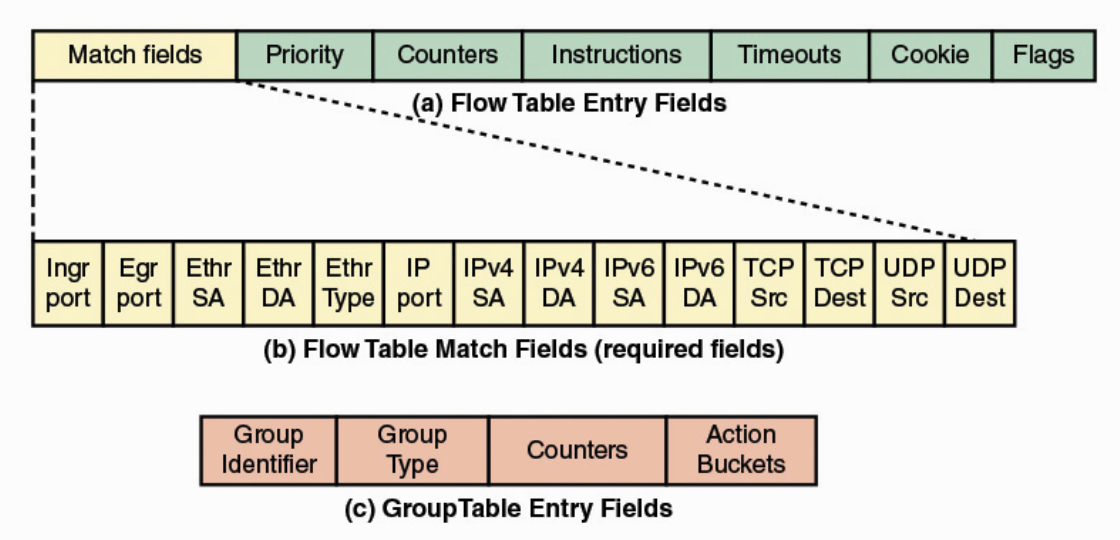
\includegraphics[width=0.95\textwidth,height=\textheight,keepaspectratio]{images/fig_4_5}
\caption{OpenFlow Table Entry Format}
\label{fig:4.5}
\end{figure}

\subsection{Flow Table Pipeline}
Uno switch include uno o pi� flow tables. Se � presente pi� di una flow table, quest'ultime sono organizzate come una pipeline, con le tabelle organizzate con numeri crescenti a partire da zero.
\newline
L'uso di tabelle multiple in una pipeline invece di una singola flow table aggiunge al controller SDN una notevole flessibilit�. 
\newline
L'OpenFlow specifica due stati di processing:
\newline
- \textbf{Ingress processing}: questo stato accade ogni volta, a cominciare dalla Tabella 0 ed utilizza l'identit� della porta di input. La Tabella 0 pu� essere anche l'unica ed in quel caso il processo � semplificato al processo di quella singola tabella e non c'� egress processing.
\newline
- \textbf{Egress processing}: � il processo che inizia dopo aver determinato la porta di output. Questo stato � opzionale ma se occorre coinvolge una o pi� tabelle. La separazione dei due stati � indicata dall'identificatore numero della prima egress table. Tutte le tabelle che hanno un numero inferiore della prima egress devono essere usate come ingress table e vicevera nessuna tabella con un numero maggiore o uguale della prima egress table pu� essere usato come ingress table.
\newline

\subsection{Group Table}
Nel corso del processo della pipeline una flow table pu� dirigere il flusso di pacchetti ad una group table o ad un'altra flow table. Le group table o le group actions abilitano l'OpenFlow a rappresentare un set di porte come una singola entit� per l'inoltro dei pacchetti. 
\newline
Differenti tipi di gruppi sono a disposizione per rappresentare differenti astrazioni di inoltro pacchetti, come il broadcasting ed il multicasting.
\newline
\newline
Ogni group table � costituita da un numero di righe, chiamate group entries, formata da quattro componenti:
\newline
- \textbf{Group Identifier}: un intero a 32 bit senza segno che unicamente identifica il gruppo. Un gruppo � definito come una entry della group table.
\newline
- \textbf{Group Type}: per determinare la semantica del gruppo.
\newline
- \textbf{Counters}: aggiornato quando i pacchetti sono processati da un gruppo.
\newline
- \textbf{Action bucket}: una lista ordinata di action bucket dove ognuna di queste contiene un set di azioni da eseguire e parametri associati. 

\section{Protocollo OpenFlow}
Il protocollo OpenFlow descrive lo scambio di messaggi che prende luogo tra l'OpenFlow Controller e l'OpenFlow Switch. Tipicamente il protocollo � implementato all'inizio del TLS per favorire un canale OpenFlow sicuro.
\newline
Il protocollo OpenFlow abilita il controller ad eseguire le azioni di add, update e delete al flusso il ingresso alla flow table. Quest'ultimo supporta tre tipi di messaggi: 
\newline
- \textbf{Controller to Switch}: questi messaggi iniziano dal controller ed in qualche caso richiedono una risposta dagli switch. Questa classe di messaggi abilita il controller a controllare lo stato logico dello switch, inclusa la sua configurazione ed i dettagli del flusso e degli ingressi nelle group table. Questo messaggio � inviato dal controller ad uno switch quando quello switch invia un pacchetto al controller ed il controller decide di non scartare il pacchetto ma di reindirizzarlo alla porta di output dello switch.
\newline
- \textbf{Asincrono}: questi tipi di messaggi sono inviati senza la sollecitazione del controller. Questa classe include vari messaggi di stato al controller. Include il messaggio di Packet-in, che pu� essere utilizzato dallo switch per inviare un pacchetto al controller quando non c'� nessun match sulla flow table.
\newline
- \textbf{Simmetrico}: questi messaggi sono inviati senza sollecitazioni ne da parte del controller ne dello switch. Sono semplici ed utili. Messaggi di "Hello" sono tipicamente inviati avanti e indietro fra il controller e lo switch quando la connessione viene stabilita. Questi messaggi di invio-risposta possono essere utilizzati sia dal controller che dallo switch per misurare la latenza, la banda, la interconnessione o per verificare che il dispositivo � online e funzionante.






